\documentclass[manuscript,nonacm]{acmart}

\usepackage{tikz}
\usepackage{amsthm}
\usepackage{subcaption}

\theoremstyle{definition}
\newtheorem{solution}{Solution}

\begin{document}

\title{Assignment~6}

\author{Yanqiao Chen}
\affiliation{%
  \institution{Southern University of Science and Technology}
  \city{Shenzhen}
  \country{China}
}
\email{12412115@mail.sustech.edu.cn}

\maketitle
\markboth{Yanqiao Chen}{Assignment~6}

\section{How to prove that $3\textsc{SAT} \leq_{P} 3\textsc{Color}$ and thus $3\textsc{Color}$ is NP-complete?}

We prove that $3\textsc{SAT} \leq_{P} 3\textsc{Color}$, which implies $3\textsc{Color}$ is NP-complete.

First, $3\textsc{Color}\in NP$.  Given a coloring of the graph, we can check every edge
and verify in polynomial time that its two endpoints receive different colors.

Now we reduce $3\textsc{Sat}$ to $3\textsc{Color}$.  We describe the construction using the
following example:
\[
  \phi=(x\vee \bar y\vee z)\wedge(\bar x\vee y\vee \bar z).
\]

The construction is built from three kinds of gadgets.  We first describe each
one in isolation and then explain how they are wired together.

\begin{figure*}[htbp]
\centering
\begin{subfigure}[b]{0.28\textwidth}
\centering
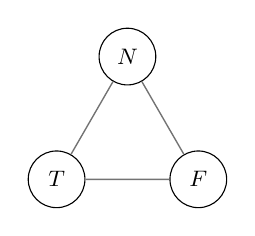
\begin{tikzpicture}[
  scale=0.9,
  transform shape,
  vertex/.style={circle, draw, minimum size=8mm, inner sep=0pt, font=\small},
  edge/.style={draw=black!55, line width=0.5pt}
]
  \node[vertex] (T) at (0,0) {$T$};
  \node[vertex] (F) at (2,0) {$F$};
  \node[vertex] (N) at (1,1.732) {$N$};
  \draw[edge] (T)--(F)--(N)--(T);
\end{tikzpicture}
\caption{Palette gadget.  The triangle forces $T,F,N$ to use three different
colours, which we interpret as True, False, and Neutral.}
\label{fig:gadget-palette}
\end{subfigure}%
\hfill
\begin{subfigure}[b]{0.32\textwidth}
\centering
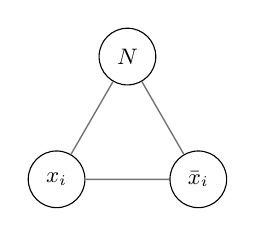
\begin{tikzpicture}[
  scale=0.9,
  transform shape,
  vertex/.style={circle, draw, minimum size=8mm, inner sep=0pt, font=\small},
  edge/.style={draw=black!55, line width=0.5pt}
]
  \node[vertex] (xi) at (0,0) {$x_i$};
  \node[vertex] (nxi) at (2,0) {$\bar x_i$};
  \node[vertex] (N) at (1,1.732) {$N$};
  \draw[edge] (xi)--(nxi)--(N)--(xi);
\end{tikzpicture}
\caption{Variable gadget.  $x_i$ and $\bar x_i$ are adjacent to each other and
to $N$, so exactly one receives the colour of $T$ and the other that of $F$.}
\label{fig:gadget-variable}
\end{subfigure}%
\hfill
\begin{subfigure}[b]{0.36\textwidth}
\centering
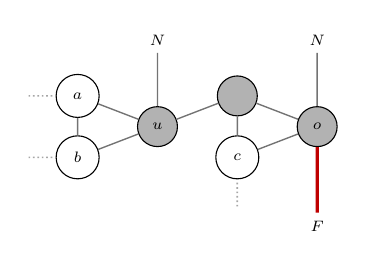
\begin{tikzpicture}[
  scale=0.78,
  transform shape,
  vertex/.style={circle, draw, minimum size=7mm, inner sep=0pt, font=\scriptsize},
  ornode/.style={circle, draw, fill=black!30, minimum size=6.5mm, inner sep=0pt, font=\scriptsize},
  edge/.style={draw=black!55, line width=0.5pt},
  restrict/.style={draw=red!75!black, line width=1.2pt},
  feed/.style={draw=black!35, densely dotted, line width=0.6pt}
]
  % First OR triangle: a OR b -> u
  \node[vertex] (a) at (0,1.8) {$a$};
  \node[vertex] (b) at (0,0.8) {$b$};
  \node[ornode] (u) at (1.3,1.3) {$u$};
  \draw[edge] (a)--(u)--(b)--(a);

  % Second OR triangle: u OR c -> o
  \node[ornode] (up) at (2.6,1.8) {};
  \node[vertex] (c) at (2.6,0.8) {$c$};
  \node[ornode] (o) at (3.9,1.3) {$o$};
  \draw[edge] (up)--(o)--(c)--(up);
  \draw[edge] (u)--(up);

  % Connections to palette
  \draw[edge] (u)--(1.3,2.5) node[above, font=\scriptsize] {$N$};
  \draw[edge] (o)--(3.9,2.5) node[above, font=\scriptsize] {$N$};
  \draw[restrict] (o)--(3.9,-0.1) node[below, font=\scriptsize] {$F$};

  % Dotted input connections
  \draw[feed] (-0.8,1.8)--(a);
  \draw[feed] (-0.8,0.8)--(b);
  \draw[feed] (2.6,0)--(c);
\end{tikzpicture}
\caption{Clause (OR) gadget for $(a\vee b\vee c)$.  Two grey triangles compute
$u=a\vee b$ and $o=u\vee c$.  Dotted edges connect literals; $u,o$ link to
$N$, and the red edge forces $o$ to be True.}
\label{fig:gadget-or}
\end{subfigure}
\caption{The three elementary gadgets.}
\label{fig:gadgets}
\end{figure*}

\paragraph{Palette gadget (Figure~\ref{fig:gadget-palette}).}
Three vertices $T,F,N$ form a triangle.  They must receive three distinct
colours, which we call True, False, and Neutral.  All other gadgets anchor to
these three vertices.

\paragraph{Variable gadget (Figure~\ref{fig:gadget-variable}).}
For each Boolean variable $x_i$ we create two vertices $x_i$ and $\bar x_i$.
Both are joined to $N$ and to each other, forming a triangle with $N$.  Because
$x_i$ and $\bar x_i$ are adjacent to $N$, neither can take the neutral colour;
because they are adjacent to each other, exactly one receives the colour of $T$
(and is interpreted as True) while the other receives the colour of $F$ (and is
interpreted as False).  Thus the gadget forces a consistent truth assignment.

\paragraph{Clause gadget (Figure~\ref{fig:gadget-or}).}
For each clause $(a\vee b\vee c)$ we chain two OR-gadgets:
\begin{enumerate}
  \item The first grey triangle has inputs $a,b$ and output $u=a\vee b$.
  \item The second grey triangle has inputs $u,c$ and output $o=u\vee c$.
\end{enumerate}
The intermediate output $u$ and the final output $o$ are each connected to the
palette vertex $N$, so both must be coloured either True or False.  The final
output $o$ is also joined to the palette vertex $F$ by a red edge.  Since $o$ is
adjacent to $F$, it cannot itself be False; therefore $o$ must be True.  The
internal structure of the OR-gadget guarantees that $o$ can be True exactly when
at least one of $a,b,c$ is True.  Hence the entire clause gadget is $3$-colourable
iff the clause is satisfied.

\paragraph{Wiring the gadgets together.}
Given a $3\textsc{Sat}$ formula $\phi$, the complete graph $G_\phi$ is assembled as
follows:
\begin{enumerate}
  \item \textbf{Add the palette.}  Insert the three palette vertices $T,F,N$ and
the edges among them.
  \item \textbf{Add variable gadgets.}  For each variable $x_i$ in $\phi$, create
vertices $x_i$ and $\bar x_i$, add the edges
$(x_i,\bar x_i)$, $(x_i,N)$, $(\bar x_i,N)$.
  \item \textbf{Add clause gadgets.}  For each clause $C_j=(a_j\vee b_j\vee c_j)$
in $\phi$, instantiate a chain of two OR-gadgets with inputs $a_j,b_j,c_j$,
intermediate output $u_j$, and final output $o_j$ as described above.  Connect
$u_j$ to $N$, connect $o_j$ to $N$, and connect $o_j$ to $F$.
  \item \textbf{Connect literals to clauses.}  Each literal vertex ($x_i$ or
$\bar x_i$) is linked by a dotted edge to every OR-gadget input that
corresponds to an occurrence of that literal in a clause.  (These dotted edges
are the only connections between the variable layer and the clause layer.)
\end{enumerate}
The construction uses a constant number of vertices and edges per variable and
per clause, so $G_\phi$ has size polynomial in $|\phi|$ and can be built in
polynomial time.

Figure~\ref{fig:3color} shows the complete graph for the example formula
$\phi=(x\vee\bar y\vee z)\wedge(\bar x\vee y\vee\bar z)$.

\begin{figure}[htbp]
\centering
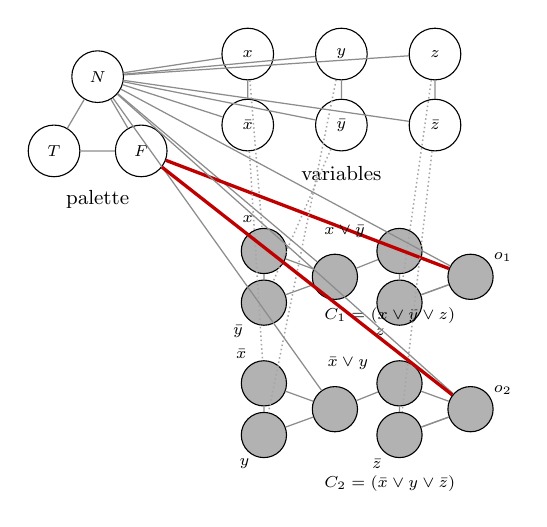
\begin{tikzpicture}[
  scale=0.82,
  transform shape,
  vertex/.style={circle, draw, minimum size=8mm, inner sep=0pt, font=\scriptsize},
  aux/.style={circle, draw, minimum size=7mm, inner sep=0pt, font=\scriptsize},
  ornode/.style={circle, draw, fill=black!30, minimum size=7mm, inner sep=0pt,
    font=\scriptsize},
  gate/.style={rectangle, draw, minimum width=13mm, minimum height=8mm,
    inner sep=1pt, font=\scriptsize},
  edge/.style={draw=black!45, line width=0.45pt},
  restrict/.style={draw=red!75!black, line width=1.2pt},
  feed/.style={draw=black!35, densely dotted, line width=0.55pt}
]
  % Palette.
  \node[vertex] (T) at (0,4.6) {$T$};
  \node[vertex] (F) at (1.35,4.6) {$F$};
  \node[vertex] (N) at (0.675,5.75) {$N$};
  \draw[edge] (T)--(F)--(N)--(T);
  \node[font=\small] at (0.675,3.85) {palette};

  % Variables.
  \node[vertex] (x) at (3.0,6.1) {$x$};
  \node[vertex] (nx) at (3.0,5.0) {$\bar x$};
  \node[vertex] (y) at (4.45,6.1) {$y$};
  \node[vertex] (ny) at (4.45,5.0) {$\bar y$};
  \node[vertex] (z) at (5.9,6.1) {$z$};
  \node[vertex] (nz) at (5.9,5.0) {$\bar z$};
  \foreach \a/\b in {x/nx,y/ny,z/nz}{
    \draw[edge] (\a)--(\b);
    \draw[edge] (\a)--(N);
    \draw[edge] (\b)--(N);
  }
  \node[font=\small] at (4.45,4.25) {variables};

  % Clause 1 complete OR-gadget chain.
  \node[ornode] (c1a) at (3.25,3.05) {};
  \node[ornode] (c1b) at (3.25,2.25) {};
  \node[ornode] (u1) at (4.35,2.65) {};
  \node[ornode] (c1u) at (5.35,3.05) {};
  \node[ornode] (c1c) at (5.35,2.25) {};
  \node[ornode] (o1) at (6.45,2.65) {};
  \draw[edge] (c1a)--(c1b)--(u1)--(c1a);
  \draw[edge] (u1)--(c1u)--(c1c)--(o1)--(c1u);
  \draw[edge] (c1c)--(o1);
  \draw[feed] (x)--(c1a);
  \draw[feed] (ny)--(c1b);
  \draw[feed] (z)--(c1c);
  \draw[edge] (u1)--(N);
  \draw[edge] (o1)--(N);
  \draw[restrict] (o1)--(F);
  \node[font=\scriptsize] at (3.0,3.55) {$x$};
  \node[font=\scriptsize] at (2.85,1.8) {$\bar y$};
  \node[font=\scriptsize] at (5.05,1.8) {$z$};
  \node[font=\scriptsize] at (4.5,3.35) {$x\vee \bar y$};
  \node[font=\scriptsize] at (6.95,2.95) {$o_1$};
  \node[font=\scriptsize] at (5.2,2.05) {$C_1=(x\vee \bar y\vee z)$};

  % Clause 2 complete OR-gadget chain.
  \node[ornode] (c2a) at (3.25,1.0) {};
  \node[ornode] (c2b) at (3.25,0.2) {};
  \node[ornode] (u2) at (4.35,0.6) {};
  \node[ornode] (c2u) at (5.35,1.0) {};
  \node[ornode] (c2c) at (5.35,0.2) {};
  \node[ornode] (o2) at (6.45,0.6) {};
  \draw[edge] (c2a)--(c2b)--(u2)--(c2a);
  \draw[edge] (u2)--(c2u)--(c2c)--(o2)--(c2u);
  \draw[edge] (c2c)--(o2);
  \draw[feed] (nx)--(c2a);
  \draw[feed] (y)--(c2b);
  \draw[feed] (nz)--(c2c);
  \draw[edge] (u2)--(N);
  \draw[edge] (o2)--(N);
  \draw[restrict] (o2)--(F);
  \node[font=\scriptsize] at (2.9,1.45) {$\bar x$};
  \node[font=\scriptsize] at (2.95,-0.25) {$y$};
  \node[font=\scriptsize] at (5.0,-0.25) {$\bar z$};
  \node[font=\scriptsize] at (4.55,1.3) {$\bar x\vee y$};
  \node[font=\scriptsize] at (6.95,0.9) {$o_2$};
  \node[font=\scriptsize] at (5.2,-0.55) {$C_2=(\bar x\vee y\vee \bar z)$};
\end{tikzpicture}
\caption{Reduction from $3\textsc{Sat}$ to $3\textsc{Color}$ for the formula
$\phi=(x\vee\bar y\vee z)\wedge(\bar x\vee y\vee\bar z)$.  Palette vertices
$T,F,N$ enforce the three colors; variable gadgets force a consistent truth
assignment; clause gadgets (gray vertices) propagate the OR of literals and
force the final output to be True via the red edges.}
\label{fig:3color}
\end{figure}

\paragraph{Correctness.}
If $\phi$ is satisfiable, colour each literal vertex according to its truth
value under a satisfying assignment (colour of $T$ for True, colour of $F$ for
False).  Because every clause has at least one true literal, each OR-gadget
can propagate True to its final output $o_j$, which is compatible with the red
edge to $F$ and the edge to $N$.  Hence $G_\phi$ admits a proper $3$-colouring.

Conversely, suppose $G_\phi$ has a proper $3$-colouring.  The variable gadgets
force each pair $(x_i,\bar x_i)$ to receive opposite non-neutral colours, so we
read off a Boolean assignment by interpreting the colour of $T$ as True.  If a
clause $C_j$ were unsatisfied under this assignment, all three of its literal
inputs would be coloured False.  The OR-gadgets would then force the final
output $o_j$ to be False as well.  But $o_j$ is adjacent to $F$ (red edge), so
$o_j$ cannot take the colour of $F$---a contradiction.  Therefore every clause
is satisfied and $\phi$ is satisfiable.

The reduction is polynomial-time because each variable and each clause
contributes only $O(1)$ vertices and edges. Thus $3\textsc{SAT} \leq_{P} 3\textsc{Color}$. Since $3\textsc{Sat}$ is NP-complete and
$3\textsc{Color}\in NP$, we conclude that $3\textsc{Color}$ is NP-complete.

\end{document}
